\documentclass[11pt]{article}

% ---------- geometry ----------
\usepackage[letterpaper,top=0.9in,bottom=0.9in,left=1in,right=1in]{geometry}

% ---------- fonts ----------
\usepackage[T1]{fontenc}
\usepackage{charter}
\usepackage[scaled=0.92]{helvet}
\usepackage{microtype}

% ---------- no hyphenation anywhere ----------
\usepackage[none]{hyphenat}
\hyphenpenalty=10000
\exhyphenpenalty=10000
\tolerance=2000
\emergencystretch=4em

% ---------- color: black, gray, white base + Solana accent ----------
\usepackage{xcolor}
\definecolor{ink}{gray}{0.13}
\definecolor{mid}{gray}{0.42}
\definecolor{soft}{gray}{0.58}
\definecolor{rulegray}{gray}{0.80}
\definecolor{fillgray}{gray}{0.90}
\definecolor{barlite}{gray}{0.78}
\definecolor{barmid}{gray}{0.52}
\definecolor{bardark}{gray}{0.17}
\definecolor{solpurple}{RGB}{124,58,237}
\definecolor{solgreen}{RGB}{18,186,122}
\color{ink}

% ---------- spacing ----------
\usepackage{parskip}
\setlength{\parskip}{0.55\baselineskip}
\usepackage{setspace}
\setstretch{1.08}

% ---------- headings with a divider rule ----------
\usepackage{titlesec}
\titleformat{\section}{\sffamily\large\bfseries\color{ink}}{\thesection}{0.7em}{}[\vspace{2.5pt}{\color{solpurple}\titlerule[0.9pt]}]
\titlespacing*{\section}{0pt}{1.35\baselineskip}{0.55\baselineskip}
\titleformat{\subsection}{\sffamily\normalsize\bfseries\color{ink}}{\thesubsection}{0.6em}{}
\titlespacing*{\subsection}{0pt}{1.0\baselineskip}{0.25\baselineskip}

% ---------- tables, lists ----------
\usepackage{booktabs}
\usepackage{array}
\usepackage{enumitem}
\setlist[itemize]{leftmargin=1.3em,itemsep=5pt,topsep=3pt,parsep=0pt}
\renewcommand{\arraystretch}{1.3}

% ---------- running header ----------
\usepackage{fancyhdr}
\pagestyle{fancy}
\fancyhf{}
\fancyhead[L]{\footnotesize\sffamily\color{soft}Boiler Blockchain \quad Purdue University}
\fancyhead[R]{\footnotesize\sffamily\color{soft}Solana (SOL) \quad Long}
\fancyfoot[C]{\footnotesize\sffamily\color{soft}\thepage}
\renewcommand{\headrule}{\color{rulegray}\hrule height 0.4pt\vspace{2pt}}
\renewcommand{\footrulewidth}{0pt}

% ---------- charts ----------
\usepackage{pgfplots}
\pgfplotsset{compat=1.18}
\usetikzlibrary{positioning}

% ---------- design helpers ----------
\newcommand{\figtitle}[1]{\par\vspace{2pt}{\sffamily\bfseries\small\color{ink} #1}\par\vspace{1pt}}
\newcommand{\figcap}[2]{\par\vspace{3pt}{\footnotesize\sffamily\color{mid}\textbf{#1}\quad #2}\par}
\newcommand{\statcell}[2]{\begin{minipage}[t]{0.235\linewidth}\centering{\sffamily\bfseries\fontsize{19}{21}\selectfont #1}\\[3pt]{\scriptsize\sffamily\color{mid}\MakeUppercase{#2}}\end{minipage}}
\newcommand{\statband}[1]{\par\vspace{7pt}{\color{solpurple}\hrule height 0.9pt}\vspace{9pt}\noindent #1 \par\vspace{9pt}{\color{solpurple}\hrule height 0.9pt}\par\vspace{4pt}}
\newcommand{\pullquote}[2]{\par\vspace{10pt}\begin{center}\begin{minipage}{0.9\linewidth}\centering{\fontsize{13.5}{17}\selectfont\color{ink}\itshape #1}\\[5pt]{\footnotesize\sffamily\color{mid}\MakeUppercase{#2}}\end{minipage}\end{center}\vspace{6pt}}

\begin{document}

% ======================= TITLE PAGE =======================
\thispagestyle{empty}
\vspace*{0.8in}

{\footnotesize\sffamily\color{soft}\MakeUppercase{Franklin Crypto Research Competition}\\[2pt]
\MakeUppercase{University Blockchain Conference 2026}}

\vspace{10pt}
{\color{solpurple}\hrule height 1.8pt}
\vspace{34pt}

{\sffamily\bfseries\fontsize{30}{34}\selectfont Buying Reliability\\ Before It Is Priced\par}

\vspace{18pt}
{\large\color{mid} An engineering and fundamental case for a long position in Solana (SOL), the settlement layer of onchain finance.\par}

\vfill

{\color{rulegray}\hrule height 0.6pt}
\vspace{16pt}

\noindent\begin{tabular}{@{}p{1.6in}l@{}}
{\sffamily\color{soft}\footnotesize AUTHOR} & Eli Dubizh \\[5pt]
{\sffamily\color{soft}\footnotesize ORGANIZATION} & Boiler Blockchain, Purdue University \\[5pt]
{\sffamily\color{soft}\footnotesize TRACK} & Long, Market Cap Over \$250M \\[5pt]
{\sffamily\color{soft}\footnotesize CONTACT} & ed200419@gmail.com \\[5pt]
{\sffamily\color{soft}\footnotesize DATE} & November 2026 \\
\end{tabular}

\vspace{20pt}
{\footnotesize\color{soft} Price and fundamentals as of early November 2026. Primary data from Blockworks Research and Allium, the competition research tools, with Anza, Messari, 21Shares, and DeFiLlama. Independent student research. Not investment advice.}

\clearpage
\setcounter{page}{1}

% ======================= 1. EXECUTIVE SUMMARY =======================
\section{Executive Summary}

We recommend a long position in Solana (SOL) at about \$89, a circulating market capitalization near \$53B. Over a 12 to 18 month horizon we see roughly 38\% downside in the bear case (\$55), roughly 80\% upside in the base case (\$160), and roughly 226\% upside in the bull case (\$290). The payoff is asymmetric because the market still prices Solana on the two variables that are weak today, memecoin era throughput and fund flows, and has not yet repriced the one that structurally changed the asset.

\statband{\statcell{\$53B}{Market cap, 69\% off high}\hfill\statcell{44$\times$}{Price to app revenue}\hfill\statcell{+48\%}{Quarterly REV growth}\hfill\statcell{150ms}{Finality, was 12.8s}}

The consensus pitch for Solana is that it is fast and cheap, and that pitch is now commoditized. Our claim is different: in a world of abundant blockspace, the scarce and value accruing resource is execution quality, uptime, deterministic finality in well under a second, and a low rate of failed transactions. The market already pays a large premium for it. Hyperliquid, a finalist in the Long over \$250M track last cycle, trades at roughly 27 times revenue precisely because it is fast, never offline, and returns about 99\% of its fees to holders. On October 21, 2026, Solana swapped its entire consensus engine in a single slot with zero downtime, a first for any live chain, cutting finality from about 12.8 seconds toward a 150 millisecond target under a hardened 20 plus 20 fault model.

\pullquote{Eighteen months of work for a migration that happens in one slot.}{Anza, on the Alpenglow upgrade}

That is the catalyst, and it converts Solana's single largest historical liability, seven outages through early 2024, into a measurable strength: nearly three years of continuous uptime. The fundamentals fit the lens this panel grades on. We will not pretend the token is statistically cheap. On raw network revenue it trades near 175 times, which looks expensive. But that denominator has broken for every base layer as blockspace became abundant, with Ethereum screening above 1,000 times on the same measure. The denominators that matter, application revenue near 44 times and reaccelerating, and the execution rerating, point the other way. You are buying a mispriced factor at a 69\% drawdown, not a cheap token.

% ======================= 2. PROJECT OVERVIEW =======================
\section{Project Overview}

\subsection{What Solana is today}
Solana is a single state, high throughput Layer 1 that settles every transaction in one global execution environment rather than fragmenting liquidity across rollups. For most of its life the bull case was performance and the bear case was reliability. In 2026 that framing is obsolete. Throughput is no longer scarce; it is a race toward zero across dozens of chains. What is scarce is a venue that institutions and high value applications can trust to be always on, fast to finality, and cheap to verify. Delphi Digital frames Solana's 2026 cycle as building a decentralized Nasdaq, an exchange grade environment where an onchain order book can compete with a centralized exchange. That is the lens this panel already uses, spanning a tokenized fund issuer, a financial infrastructure fund, and the research firm that defined the network revenue metric.

\subsection{The engineering turn: Alpenglow}
Alpenglow is the largest change to Solana since launch, and the detail matters because this is an engineering thesis. It replaces the previous consensus, TowerBFT, with Votor, a new voting and finality path built on aggregated signatures and a two round design that finalizes a block in one round at or above 80\% participation. Votes move off the chain, which both collapses finality and frees an estimated 70\% of the block space that vote transactions used to consume. The new fault model keeps finalizing through 20\% malicious and 20\% offline stake at the same time, a materially stronger guarantee than the old threshold below 33\%. The migration itself is the proof: Anza executed an eighteen month build as a one slot swap on live mainnet with zero downtime, the first time any network has replaced its consensus engine without halting. This is a dated, verifiable milestone, not a roadmap promise. The whole reliability argument sits in four numbers: seven halts between December 2020 and February 2024, a last outage on February 6, 2024, nearly three years of continuous uptime since, and finality compressed from about 12.8 seconds toward 150 milliseconds.

\subsection{The economic engine}
Strip away the narrative and Solana is, by the metrics this competition rewards, the most economically active base layer in crypto. It has led all chains in application revenue for nine consecutive quarters, printed about \$299M in the third quarter of 2026, and carries the deepest onchain stablecoin base outside Ethereum and Tron at a record near \$16.8B. Network revenue collapsed about 87\% as the memecoin cycle unwound, and then rose 48\% over the prior quarter in Q3 2026, its first increase in six quarters. That inflection, off a washed out base, is the signal that the franchise is broadening into payments, decentralized finance, and tokenized assets.

\figtitle{Figure 1 \quad Network revenue washed out, then inflected, while apps kept earning}
\begin{center}
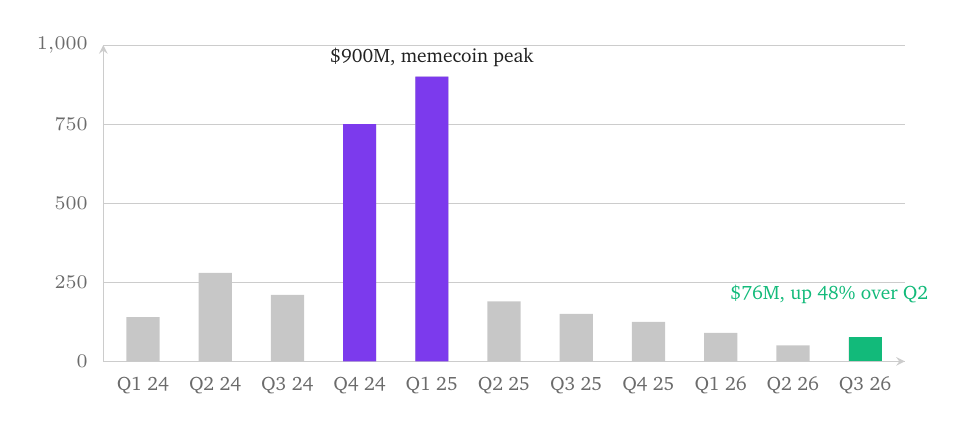
\begin{tikzpicture}
\begin{axis}[
  width=0.97\linewidth, height=5.6cm,
  ybar, bar width=12pt, bar shift=0pt,
  ymin=0, ymax=1000,
  axis x line=bottom, axis y line=left,
  x axis line style={draw=rulegray}, y axis line style={draw=rulegray},
  xtick=data, tick style={draw=none},
  symbolic x coords={Q1 24,Q2 24,Q3 24,Q4 24,Q1 25,Q2 25,Q3 25,Q4 25,Q1 26,Q2 26,Q3 26},
  xticklabel style={font=\scriptsize\color{mid}},
  ytick={0,250,500,750,1000}, yticklabel style={font=\scriptsize\color{mid}},
  ymajorgrids, major grid style={draw=rulegray,line width=0.2pt},
  enlarge x limits=0.055, clip=false,
]
\addplot[draw=none,fill=barlite] coordinates {(Q1 24,140)(Q2 24,280)(Q3 24,210)(Q4 24,750)(Q1 25,900)(Q2 25,190)(Q3 25,150)(Q4 25,125)(Q1 26,90)(Q2 26,51)(Q3 26,76)};
\addplot[draw=none,fill=solpurple] coordinates {(Q4 24,750)(Q1 25,900)};
\addplot[draw=none,fill=solgreen] coordinates {(Q3 26,76)};
\node[font=\scriptsize,text=ink,anchor=south] at (axis cs:Q1 25,900) {\$900M, memecoin peak};
\node[font=\scriptsize,text=solgreen,anchor=south west] at (axis cs:Q1 26,150) {\$76M, up 48\% over Q2};
\end{axis}
\end{tikzpicture}
\figcap{Figure 1.}{Solana quarterly network revenue, fees plus validator tips, USD millions. The purple bars are the memecoin era peak; the green bar is the Q3 2026 inflection. Application revenue, a separate line near \$1.2B annualized, stayed first across all chains throughout. Source: Blockworks Research.}
\end{center}

\subsection{Token, value accrual, catalysts, and risks}
SOL has about 590 million tokens circulating of roughly 636 million total, issuance near 3.6\% and disinflating, and about 68\% of supply staked, close to \$38B of economic security. Value reaches the token through fees and validator tips paid to stakers, a protocol burn, and the staking yield. Demand is structurally new: staking enabled spot funds from Franklin Templeton and Bitwise hold more than \$1.3B and are removing float faster than issuance adds it.

\textbf{Catalysts and risks.}
\begin{itemize}
  \item \textbf{Catalysts.} The reliability rerating as the zero outage record compounds; rising Firedancer stake share; staking enabled fund inflows; tokenized equities and real world assets, with Franklin's own money market fund already settling on Solana.
  \item \textbf{Risks.} Rich on network revenue, which we answer with application revenue and the rerating; client concentration, which Firedancer is actively fixing; geographic stake concentration near 59\%, a genuine open risk; and near term price and flow weakness, already discounted by a 69\% drawdown.
\end{itemize}

% ======================= 3. INVESTMENT PROPOSAL =======================
\section{Investment Proposal}

Position: long Solana. Entry near \$89. Horizon: 12 to 18 months. Base case exit near \$160. The thesis resolves as the market rerates Solana from a memecoin beta Layer 1 into an execution grade settlement layer, while application revenue compounds and net float shrinks. The two charts below frame it: what the market pays for execution quality, and where a rerating leads.

\vspace{2pt}
\noindent
\begin{minipage}[t]{0.5\linewidth}
\figtitle{What the market pays for execution}
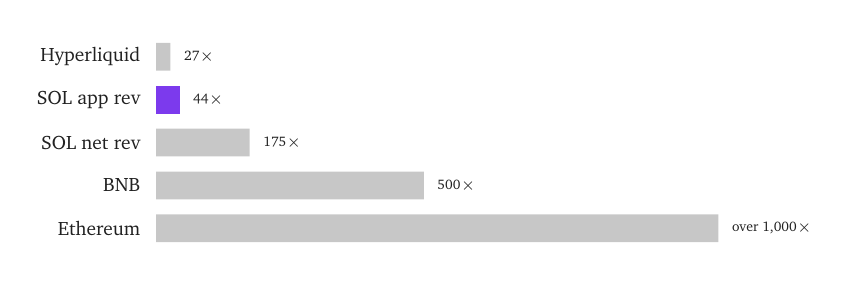
\begin{tikzpicture}
\begin{axis}[
  width=\linewidth, height=4.5cm,
  xbar, bar width=10pt, bar shift=0pt,
  xmin=0, xmax=1550,
  axis x line=none, axis y line=left,
  y axis line style={draw=none}, ytick style={draw=none},
  symbolic y coords={Ethereum,BNB,SOL net rev,SOL app rev,Hyperliquid},
  ytick={Ethereum,BNB,SOL net rev,SOL app rev,Hyperliquid},
  yticklabel style={font=\scriptsize\color{ink}},
  enlarge y limits=0.17, clip=false,
]
\addplot[draw=none,fill=barlite] coordinates {(27,Hyperliquid)(175,SOL net rev)(500,BNB)(1050,Ethereum)};
\addplot[draw=none,fill=solpurple] coordinates {(44,SOL app rev)};
\node[right,font=\tiny,text=ink] at (axis cs:27,Hyperliquid) {\;27$\times$};
\node[right,font=\tiny,text=ink] at (axis cs:44,SOL app rev) {\;44$\times$};
\node[right,font=\tiny,text=ink] at (axis cs:175,SOL net rev) {\;175$\times$};
\node[right,font=\tiny,text=ink] at (axis cs:500,BNB) {\;500$\times$};
\node[right,font=\tiny,text=ink] at (axis cs:1050,Ethereum) {\;over 1,000$\times$};
\end{axis}
\end{tikzpicture}
\par\vspace{1pt}{\scriptsize\sffamily\color{mid} Price to revenue by chain. Lower is cheaper.}
\end{minipage}\hfill
\begin{minipage}[t]{0.46\linewidth}
\figtitle{The rerating path}
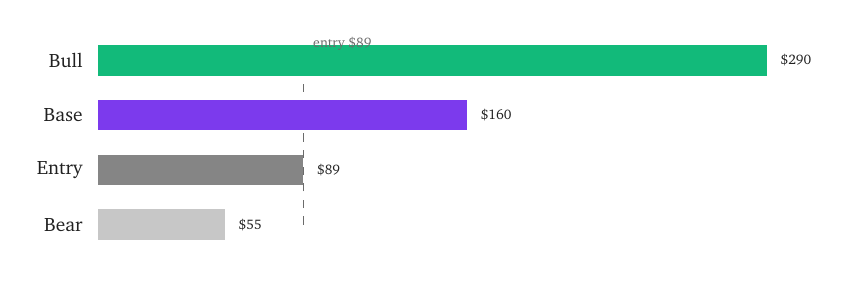
\begin{tikzpicture}
\begin{axis}[
  width=\linewidth, height=4.5cm,
  xbar, bar width=11pt, bar shift=0pt,
  xmin=0, xmax=360,
  axis x line=none, axis y line=left,
  y axis line style={draw=none}, ytick style={draw=none},
  symbolic y coords={Bear,Entry,Base,Bull}, ytick={Bear,Entry,Base,Bull},
  yticklabel style={font=\scriptsize\color{ink}},
  enlarge y limits=0.2, clip=false,
]
\draw[dashed,draw=mid,line width=0.6pt] (axis cs:89,Bear) -- (axis cs:89,Bull);
\addplot[draw=none,fill=barlite] coordinates {(55,Bear)};
\addplot[draw=none,fill=barmid] coordinates {(89,Entry)};
\addplot[draw=none,fill=solpurple] coordinates {(160,Base)};
\addplot[draw=none,fill=solgreen] coordinates {(290,Bull)};
\node[right,font=\tiny,text=ink] at (axis cs:55,Bear) {\;\$55};
\node[right,font=\tiny,text=ink] at (axis cs:89,Entry) {\;\$89};
\node[right,font=\tiny,text=ink] at (axis cs:160,Base) {\;\$160};
\node[right,font=\tiny,text=ink] at (axis cs:290,Bull) {\;\$290};
\node[font=\tiny,text=mid,anchor=south west] at (axis cs:89,Bull) {entry \$89};
\end{axis}
\end{tikzpicture}
\par\vspace{1pt}{\scriptsize\sffamily\color{mid} Scenario prices against the \$89 entry.}
\end{minipage}
\figcap{Figure 2.}{Left, price to annualized revenue; Hyperliquid uses protocol revenue, the base layers use network revenue, and the purple bar is Solana on application revenue, about 44 times. Right, the scenario targets. Source: Blockworks Research, DeFiLlama.}

\subsection{Valuation on the metrics that matter}
We value Solana through three lenses that converge. First, reframe the multiple: on network revenue SOL screens near 175 times, but that metric has broken for every base layer, and the economically meaningful number is price to application revenue near 44 times on about \$1.2B annualized, and growing. Second, price the factor: the market pays about 27 times revenue for Hyperliquid's execution quality, and Alpenglow qualifies Solana for the same factor at base layer scale and far greater diversification. Third, weigh supply and demand: staking enabled funds, treasury accumulation, and roughly 68\% of supply staked are removing float faster than issuance near 3.6\% adds it. A probability weighting of 25\% bear, 50\% base, and 25\% bull implies an expected value near \$166, about 87\% above the entry.

\subsection{Why this is the trade}
The consensus pitch, price and throughput and fund flows, is weak right now, which is the opportunity, because the market is watching lagging variables. Reliability and execution quality are the variables that rerate assets. The market proved it with Hyperliquid, and they inflected for Solana on October 21. We are positioned in front of the rerating rather than behind it.

% ======================= 4. CONCLUSION =======================
\section{Conclusion}

Solana spent four years being judged on the thing it did worst, staying online. On October 21, 2026 it retired that liability in a single slot, and in doing so it changed what kind of asset it is: from a high beta throughput bet into the only base layer at \$50B scale that can credibly claim exchange grade reliability and finality in well under a second. The market has not repriced that, because it is still watching memecoin revenue and fund flows, both near cyclical lows, rather than the variable that actually drives revaluations. We know the market pays for execution quality because it already does, and Alpenglow makes the same case for Solana on a franchise with nine quarters of leading application revenue, a record stablecoin base, and a freshly inflecting revenue line. Buying near \$89, roughly 69\% below the prior high and three weeks after the catalyst, is buying a mispriced factor with the downside already discounted.

\textbf{Recommendation: long Solana over a 12 to 18 month horizon. Base target \$160, about 80\% upside. Bull target \$290. Bear target \$55. The reliability is proven. The rerating is not yet priced. That gap is the trade.}

\vspace{14pt}
{\color{solpurple}\hrule height 0.9pt}
\vspace{10pt}
\noindent
\begin{minipage}[t]{0.31\linewidth}\centering{\sffamily\bfseries\fontsize{18}{20}\selectfont (38\%)}\\[3pt]{\scriptsize\sffamily\color{mid}\MakeUppercase{Bear, SOL \$55}}\end{minipage}\hfill
\begin{minipage}[t]{0.31\linewidth}\centering{\sffamily\bfseries\fontsize{18}{20}\selectfont +80\%}\\[3pt]{\scriptsize\sffamily\color{mid}\MakeUppercase{Base, SOL \$160}}\end{minipage}\hfill
\begin{minipage}[t]{0.31\linewidth}\centering{\sffamily\bfseries\fontsize{18}{20}\selectfont +226\%}\\[3pt]{\scriptsize\sffamily\color{mid}\MakeUppercase{Bull, SOL \$290}}\end{minipage}
\vspace{10pt}
{\color{solpurple}\hrule height 0.9pt}

% ======================= APPENDIX =======================
\clearpage
\section*{Appendix}

{\small\sffamily\color{mid}\textbf{Valuation comparables, November 2026}}
\vspace{-2pt}

\begin{center}
\begin{tabular}{@{}lllll@{}}
\toprule
{\sffamily\footnotesize\color{mid}CHAIN} & {\sffamily\footnotesize\color{mid}CAP} & {\sffamily\footnotesize\color{mid}ANNUAL REV} & {\sffamily\footnotesize\color{mid}PRICE / REV} & {\sffamily\footnotesize\color{mid}STABLECOINS} \\
\midrule
Solana & \$53B & \$0.30B & about 175 times & \$16.8B \\
Ethereum & \$280B & about \$0.26B & above 1,000 times & \$137B \\
BNB Chain & \$95B & about \$0.18B & about 500 times & \$13.8B \\
TRON & \$31B & about \$0.30B & about 100 times & \$89B \\
Hyperliquid & about \$19B & about \$0.70B & about 27 times & \$6.4B \\
\bottomrule
\end{tabular}
\end{center}

{\footnotesize\color{mid} Hyperliquid uses protocol revenue, the metric its token captures through buybacks, the correct lens for an application chain and the execution comparison. The base layer rows use network revenue, fees plus validator tips. On an application revenue basis Solana trades near 44 times. Source: Blockworks Research and DeFiLlama.}

\vspace{10pt}
{\small\sffamily\color{mid}\textbf{Alpenglow, before and after}}
\vspace{-2pt}

\begin{center}
\begin{tabular}{@{}lll@{}}
\toprule
{\sffamily\footnotesize\color{mid}DIMENSION} & {\sffamily\footnotesize\color{mid}BEFORE} & {\sffamily\footnotesize\color{mid}AFTER} \\
\midrule
Consensus & TowerBFT & Votor \\
Finality & about 12.8 seconds & target near 150 milliseconds \\
Fault model & below 33\% & 20\% plus 20\% \\
Votes & on the chain & off the chain \\
Validator cost & baseline & about 60\% lower \\
Uptime & seven halts & continuous for nearly three years \\
\bottomrule
\end{tabular}
\end{center}

{\footnotesize\color{mid} Live on mainnet on October 21, 2026, at epoch 1064, slot 459,653,000. Rotor, the propagation layer, is still pending and treated as upside. Live finality measured near 430 milliseconds in October 2026. Source: Anza, Messari, Helius. Data note: network revenue, application revenue, stablecoin supply, and market cap are drawn from the Blockworks Research blockchains dataset, the competition tool, where network revenue equals base plus priority fees plus validator tips, cross checked against the Blockworks Solana third quarter 2026 report and 21Shares. Annualized figures use the Q3 2026 run rate.}

% ======================= REFERENCES =======================
\section*{References}

\begin{enumerate}[leftmargin=1.5em,itemsep=2pt,topsep=2pt]
  \item Blockworks Research. Blockchains dataset and Solana third quarter 2026 token holder report, and the real economic value methodology.
  \item Anza. Alpenglow upgrade and mainnet activation. anza.xyz and solana.com.
  \item Messari. Solana October 2026 update and measured finality.
  \item Helius and Syndica. Alpenglow technical explainers, covering Votor, Rotor, and the fault model.
  \item 21Shares. Solana first half 2026 network revenue.
  \item DeFiLlama. Hyperliquid fees and revenue, cross chain exchange volume, and total value locked.
  \item Delphi Digital. Solana as a decentralized Nasdaq, January 2026.
  \item Franklin Templeton. Franklin Solana fund and the BENJI money market fund on Solana.
  \item Bitwise. Solana staking report, third quarter 2026, and the spot Solana fund.
  \item CoinDesk and The Block. Hyperliquid revenue, buybacks, and market share, 2026.
\end{enumerate}

\end{document}
